\chapter{Introducción}
\begin{center}
	En este capítulo se presenta una introducción a las formas\\ 		
	cuadráticas, sus representaciones y su clasificación \citep{AbarcaSoteloMarioAlberto2011Apds}.
\end{center}

\section{FORMAS CUADRÁTICAS}

\paragraph*{}
Esta sección fue adaptada de \citep{LayDavidC2001Alys}. Algunas demostraciones aquí omitidas pueden consultarse en dicha referencia.\\
Fijamos un conjunto de variables $\{x_1, x_2, \ldots, x_n\}$. Un \textbf{monomio} es un producto de la forma $x_{1}^{e_{1}} \cdot x_{2}^{e_{2}} \cdots x_{n}^{e_{n}}$ donde cada $e_{i}$ es un número natural. Un \textbf{término} se forma al multiplicar a un monomio por una constante, a la cual llamamos \textbf{coeficiente} del término. Un \textbf{polinomio} es una suma finita de términos.\\
Ejemplo: $7x^{2}y + 5x^z{4} - y$ es un polinomio sobre las variables $x$, $y$ y $z$ con tres monomios: $x^{2}y$, $xz^{4}$ y $y$ cuyos respectivos coeficientes son $2$, $4$, $1$ respectivamente.\\
Todo polinomio sobre $n$ varialbles es una función con dominio $\mathbb{R}^{n}$ y rango $\mathbb{R}$. Una \textbf{forma cuadrática} es un polinomio $q : \mathbb{R}^{n} \rightarrow \mathbb{R}$(con $n > 0$) si cada monomio del mismo es una variable al cuadrado o la multiplicación de dos variables. Esto es equivalente a decir que $q$ se puede expresar como

\begin{equation*}
q(x_{1}, x_{2}, \ldots, x_{n}) = \sum_{i=1}^{n} q_{ii}x_{i}^{2}+ \sum_{j=2}^{n}\sum_{i=1}^{j-1} q_{ij}x_{i}x_{j}
\end{equation*}

\paragraph*{}
Los ejemplos más usuales aparecen al lado izquierdo del signo igual de las ecuaciones en las cónicas con centro en el origen

\begin{equation*}
ax^{2} + 2bxy + cy^{2} = d
\end{equation*}

\paragraph*{}
y de las superficies cuadráticas con centro en el origen

\begin{equation*}
ax^{2} + 2dxy + 2exz + by^{2} + 2fyz + cz^{2} = g
\end{equation*}

\paragraph*{}
donde $a$, $b$, $c$, $d$, $e$, $f$ y $g$ son números reales. Este tipo de polinomios surgen de manera natural en diversas áreas de la ingeniería, procesamiento de señales, cinética, economía, geometría diferencial y estadística.\\
En algunos curso básicos de álgebra lineal se suele definir el concepto de forma cuadrática como una función que se puede escribir como

\begin{equation*}
q(\overrightarrow{x}) = \frac{1}{2} \overrightarrow{x}^{T} A \overrightarrow{x}
\end{equation*}

\paragraph*{}
para alguna matriz simétrica $A$. En realidad esta representación matricial es equivalente a nuestra definición con monomios; a continuación veremos como pasar de una representación a otra. Primero notemos que $\frac{1}{2} \overrightarrow{x}^{T} A \overrightarrow{x}$ se puede reescribir como sigue:

\begin{align*}
\frac{1}{2} \overrightarrow{x}^{T} A \overrightarrow{x} &= \frac{1}{2}[x_{1}, x_{2},\ldots,x_{n}] 
\begin{bmatrix}
a_{11} & a_{12} & \cdots & a_{1n}\\
a_{21} & a_{22} & \cdots & a_{2n}\\
\vdots & \vdots & \ddots & \vdots \\
a_{n1} & a_{n2} & \cdots & a_{nn}
\end{bmatrix} 
\begin{bmatrix}
x_{1}\\
x_{2}\\
\vdots\\
x_{n}
\end{bmatrix} \\ 
&= \frac{1}{2} \left[\sum_{i=1}^{n} a_{i1}x_{i}, \sum_{i=1}^{n} a_{i2}x_{i}, \ldots , \sum_{i=1}^{n} a_{in}x_{i} \right] 
\begin{bmatrix}
x_{1}\\
x_{2}\\
\vdots\\
x_{n}
\end{bmatrix} \\ 
&=   \frac{1}{2} \left[\sum_{i=1}^{n} a_{i1}x_{i}x_{1} + \cdots + \sum_{i=1}^{n} a_{in}x_{i}x_{n}\right]\\ 
&=   \frac{1}{2} \sum_{i=1}^{n}\sum_{j=1}^{n} a_{ij}x_{i}x_{j}
\end{align*}

\paragraph*{}
Al desarrollar esto se puede ver que el coeficiente de $x_{i}$ $x_{j}$ es $q_{ij} = \frac{1}{2} \left(a_{ij} + a_{ji} \right)$ porque $x_{i}$ $x_{j}$ = $x_{j}$ $x_{i}$, pero como dijimos que $A$ es simétrica $\left( a_{ij} = a_{ji}\right)$ entonces $q_{ij} = a_{ij}$. En particular cuando $i = j$ se tiene que el coeficiente de $x_{i}^{2}$ es $q_{ii} = \frac{1}{2}a_{ii}$. Por lo cuál tenemos la siguiente identidad:

\begin{equation}
    \frac{1}{2} \overrightarrow{x}^{T} A \overrightarrow{x} = \sum_{i=1}^{n}\frac{1}{2} a_{ii}x_{i}^{2} + \sum_{j=2}^{n}\sum_{i=1}^{j-1} a_{ij}x_{i}x_{j}
    \label{ecuacion:1.1}
\end{equation}

\paragraph*{}
La matriz simétrica $A$ de esta identidad se conoce como \textbf{matriz asociada a la forma cuadrática $q$}. Se denota por \textbf{$A_{q}$}, y según la ecuación  \ref{ecuacion:1.1} se puede calcular como sigue:

\begin{equation}
a_{ij} = \left \{ 
    \begin{matrix} 
    q_{ij} & \mbox{si } i < j\\
    2q_{ij} & \mbox{si } i = j\\ 
    q_{ji} & \mbox{si } i > j
    \end{matrix}\right.
    \label{ecuacion:1.2}
\end{equation}

\paragraph*{}
Por ejemplo, para $q(x, y, x) = 6x^{2} + 2y^{2} + 4z^{2} - 2xy + 10xz - 6yz$

\begin{equation*}
q(x. y. z) = = \frac{1}{2}\left[x ~  y ~ z\right] 
\begin{bmatrix}
12 & -2 & 10\\
-2 & 4 & -6\\
10 & -6 & 8
\end{bmatrix}
\begin{bmatrix}
x\\
y\\
z\\
\end{bmatrix}
\end{equation*}

\paragraph*{}
\textbf{CAMBIO DE VARIABLE}

\paragraph*{}
Un \textbf{cambio de variable} es una ecuación de la forma

\begin{equation}
    \begin{matrix} 
    \overrightarrow{x} = P\overrightarrow{y} & \mbox{o bien } & \overrightarrow{y} = P^{-1}\overrightarrow{x}\\
    \end{matrix}.
    \label{ecuacion:1.3}
\end{equation}

\paragraph*{}
donde $P$ es una matriz invertible y $\overrightarrow{y}$ es un nuevo vector variable en $\mathrm{R}^{n}$. Si se aplica el cambio de variable \ref{ecuacion:1.3} sobre una forma cuadrática $q(\overrightarrow{x}) = \frac{1}{2}\overrightarrow{x}^{T}A\overrightarrow{x}$ se obitene una matriz cuadrática $q'(\overrightarrow{y})$ cuya matriz asociada es $P^{T} ~ A ~ P$:

\begin{equation*}
    \frac{1}{2}\overrightarrow{x}^{T}\overrightarrow{x} = \frac{1}{2}\left(P\overrightarrow{y}\right)^{T}~A~\left(P\overrightarrow{y}\right) = \frac{1}{2}\left(\overrightarrow{y}^{T} P^{T}\right)~A~\left(P\overrightarrow{y}\right) = \frac{1}{2}\overrightarrow{y}^{T}\left(P^{T}~A~P\right)\overrightarrow{y}
\end{equation*}.

\paragraph*{}
Gatantizamos que $P^{T}~A~P$ es una matriz simétrica (y por tanto que en verdad corresponde a otra forma cuadrática) porque

\begin{eqnarray*}
\left(P^{T}~A~P\right)^{T}&=&P^{T}~A^{T}~\left(P^{T}\right)^{T}\\
&=&P^{T}~A^{T}~P\\
&=&P^{T}~A~P
\end{eqnarray*}

\paragraph*{}
Mediante el cambio de variable $\overrightarrow{y} = P~\overrightarrow{x}$ tenemos que $q(\overrightarrow{x}) = q'(\overrightarrow{y})$ y diremos que $q$ y $q'$ son \textbf{equivalentes} mediante la matriz invertible $P$. Si denotamos $\overrightarrow{y} = L(\overrightarrow{x})$(es decir, $L(\overrightarrow{x}) = P\overrightarrow{x})$ entonces $q'(\overrightarrow{y}) = q'\left(L(\overrightarrow{x})\right) = \left(q' \circ L\right)(\overrightarrow{x})$, por lo tanto

\begin{equation*}
q' = q \circ L
\end{equation*}

\begin{example}
Consideremos la forma cuadrática $x^{2} - 5y^{2} - 8xy$ con matriz asociada
\begin{equation*}
    \begin{matrix} 
    A = \begin{bmatrix}
2 & -8\\
-8 & 10
\end{bmatrix}
    \end{matrix}.
\end{equation*}
y el cambio de variable definido por
\begin{equation*}
    \begin{matrix} 
    \begin{bmatrix}
        x\\
        y
    \end{bmatrix} = \begin{bmatrix}
    \frac{2}{\sqrt(5)} & \frac{1}{\sqrt(5)}\\
    -\frac{1}{\sqrt(5)} & \frac{2}{\sqrt(5)}
    \end{bmatrix}\begin{bmatrix}
    z\\
    w
    \end{bmatrix} = \begin{bmatrix}
        \frac{2z + w}{\sqrt(5)}\\
        \frac{-z + 2w}{\sqrt(5)}
        \end{bmatrix}
    \end{matrix}.
\end{equation*}

La matriz $ \begin{matrix} 
    P = \begin{bmatrix}
\frac{2}{\sqrt(5)} & \frac{1}{\sqrt(5)}\\
-\frac{1}{\sqrt(5)} & \frac{2}{\sqrt(5)}
\end{bmatrix}
    \end{matrix}$ es invertible, y su inversa es 

\begin{equation*}
    \begin{matrix} 
    P^{-1} = \begin{bmatrix}
\frac{2}{\sqrt(5)} & -\frac{1}{\sqrt(5)}\\
\frac{1}{\sqrt(5)} & \frac{2}{\sqrt(5)}
\end{bmatrix}
    \end{matrix} = P^{T}
\end{equation*}

Calculamos $ \begin{matrix} 
    P^{T}~A~P = \begin{bmatrix}
6 & 0\\
0 & -14
\end{bmatrix}
    \end{matrix}$ para concluir que 
\begin{equation*}
x^{2} - 5y^{2} - 8xy = 3z^{2} - 7w^{2}
\end{equation*}

Esto es lo que se hubiese obtenido de hacer las sustituciones 

\begin{eqnarray*}
x & \leftarrow & \frac{2z + w}{\sqrt(5)}\\
y & \leftarrow & \frac{-z + 2w}{\sqrt(5)}
\end{eqnarray*}

sobre la expresion $x^{2} - 5y^{2} - 8xy$.
\end{example}

\paragraph*{}
Las cosas a destacar en este ejemplo son:
\begin{itemize}
    \item $P$ resultó ser una \textbf{matriz ortogonal}, en otras palabras, $P^{-1} = P^{T}$.
    \item $A$ es una matriz \textbf{ortogonalmente diagonizable}, en otras palabras, existe una matriz ortogonal $P$ tal que $P^{-1}~A~P$ es una matriz diagonal.
\end{itemize}

\begin{theorem}
Toda matriz es ortogonalmente diagonizable si y solo si es simétrica
\label{teorema:1.1}
\end{theorem}

\paragraph*{}
El teorema \ref{teorema:1.1} se dejara sin demostración. Lo importante es que, a partir de este teorema, y dado que las matrices asociadas a las formas cuadráticas son simëtricas, se sigue el siguente resultado:

\begin{theorem}(de los ejes principales).
Toda forma cuadrática $q(\overrightarrow{x})$ es equivalente mediante una matriz ortogonal $P$ a una forma cuadrática 
\begin{equation}
    q'(\overrightarrow{y}) = \lambda_{1}y_{1}^{2} + \lambda_{2}y_{2}^{2} + \cdots + \lambda_{n}y_{n}^{2}
\end{equation}
\label{teorema:1.2}
\end{theorem}

\begin{proof}
La matriz $A$ asociada a $q$ es simétrica, luego por teorema anterior existe una matriz $P$ tal que 
\begin{equation*}
    P^{-1}~A~P = \begin{bmatrix}
    \lambda_{1} & &\\
    & \ddots & \\
    & & \lambda_{n}
    \end{bmatrix}
    \label{ecuacion:1.4}
\end{equation*}

Haciendo $\overrightarrow{x} = P\overrightarrow{y}$ y se obtiene $q'(\overrightarrow{y}) = \frac{1}{2}\overrightarrow{y}^{T}\left(P^{T}~A~P\right)\overrightarrow{y} = \lambda_{1}y_{1}^{2} + \lambda_{2}y_{2}^{2} + \cdots + \lambda_{n}y_{n}^{2}$

\end{proof}

\paragraph*{}
Como se vera, esta representación es muy útil para clasificar formas cuadráticas. Diremos que una forma cuadrática $q$ es \textbf{definida positiva} si $q(\overrightarrow{x}) > 0, ~\forall~ \overrightarrow{x} \neq \overrightarrow{0}$ 

\begin{lemma}
Si dos formas cuadráticas $q(\overrightarrow{x})$ y $q'(\overrightarrow{y})$ son equivalentes mediante el cabio de variable $\overrightarrow{y} = P\overrightarrow{x}$ y si una de ellas es definada positiva entonces la otra también lo es.
\label{lema:1.3}
\end{lemma}

\begin{proof}
Supongamos que $q(\overrightarrow{x})$ es definida positiva y definimos la transformación lineal $L(\overrightarrow{x}) = P\overrightarrow{x}$, entonces $L(\overrightarrow{0}) = L(\overrightarrow{0}+ \overrightarrow{0}) = L(\overrightarrow{0}) + L(\overrightarrow{0})$, de donde $L(\overrightarrow{0}) = \overrightarrow{0}$. Como $P$ es una matriz invertible entonces $L^{-1}(\overrightarrow{x}) = P^{-1}x$. En particular $L$ debe ser inyectiva y por lo tanto $L(\overrightarrow{x})=\overrightarrow{0}$ implica que $\overrightarrow{x}=\overrightarrow{0}$. SI $q$ es definida positiva entonces $q(\overrightarrow{x}) = q'(\overrightarrow{y}) > 0$ para todo $\overrightarrow{x} \neq 0$; por lo tanto $q'$ es definida positiva , entonces aplicando el mismo razonamiento con $L(\overrightarrow{y}) = P^{-1}\overrightarrow{y}$ se llega a la conclusión de que $q$ tambien es definida positiva. 
\end{proof}

\begin{theorem}
Sea $q$ una forma cuadrática y supongamos que 
\begin{equation*}
q \left(\overrightarrow{x}\right) = q'(y) = \lambda_{1}y_{1}^{2} + \lambda_{2}y_{2}^{2} + \cdots + \lambda_{n}y_{n}^{2}
\end{equation*}
entonces $q$ es definida positiva si y solo si todos los $\lambda_{i} > 0$
\label{teorema:1.4}
\end{theorem}

\begin{proof}
Por el lema anterior $q$ es definida positiva si y solo si $q'$ es definida positiva. Por contradicción, si $\lambda_{i} \leq 0$ entonces definimos $y' = (y_{1}, y_{2}, \ldots, y_{n})$ donde todos los $y_{k}=0$ excepto $y_{i} = 1$. Claramente $\overrightarrow{y} \neq \overrightarrow{0}$ pero $q(\overrightarrow{y}) = \lambda_{i} \leq 0$; por lo tanto $q$ no es definida positiva.
\end{proof}

\paragraph{}
Como las formas cuadráticas se pueden representar mediante matrices entonces podemos decir que una matriz $A$ es definida positiva si su forma cuadrática asociada $q(\overrightarrow{x}) = \frac{1}{2}\overrightarrow{x}^{T}A\overrightarrow{x}$ es definida positiva.

\paragraph{}
El siguiente teorema típico de los cursos de análisis numérico nos da un criterio computacionalmente eficiente para decidir cuando una matriz simétrica es definida positiva(sin demostración).

\begin{theorem}
Una matriz $A$ es definida positiva si y solo si tiene \textbf{factorización de Cholesky}, es decir, se puede escribir como $A=R^{T}R$ donde $R$ es una matriz triangula superior con entradas positivas.
\label{teorema:1.5}
\end{theorem}

\section{FORMAS UNITARIAS}
\paragraph*{}
Esta sección fue adaptada de \citep{Ringel1985TameAA} y \citep{alma991031505829703276}. Las \textbf{formas cuadráticas enteras} son un caso especial de las formas cuadráticas donde todos los coeficientes $q_{ij}$ son todos números enteros. Si además exigimos que $q_{ii} = 1$ para $i = 1, 2, \ldots, n$ entonces las llamamos \textbf{formas cuadráticas unitarias}. En el resto de este trabajo solo se trabaja con formas cuadráticas enteras que son unitarias por lo que  las llamaremos \textbf{formas unitarias} en adelante a las que son cuadráticas y enteras.

\paragraph*{}
\textbf{CAMBIO DE VARIABLE ENTERO}

\paragraph*{}
Una \textbf{matriz entera $M$} es una matriz tal que todas sus entradas son números enteros, y es $\mathbb{Z}$\textbf{-invertible} si además su matriz inversa $M^{-1}$ tambien es una matriz entera. Un \textbf{cambio de variable entero} es un cambio de variable $\overrightarrow{y} = P\overrightarrow{x}$ donde $P$ es una matriz $\mathbb{Z}$-invertible. Los cambios de variables enteros tienen la propiedad de que transforman formas cuadráticas enteras en formas cuadráticas enteras(demostración: sean $A$ y $P$ matrices enteras, entonces $P^{T}~A~P$ es una matriz entera). Cuando $q(\overrightarrow{x}) = q'(\overrightarrow{y})$ mediante el cambio de variable entero $\overrightarrow{y} = P\overrightarrow{x}$ diremos que $q$ y $q'$ son $\mathbb{Z}$-\textbf{equivalentes} mediante la matriz $\mathbb{Z}$-invertible $P$.

\paragraph*{}
\textbf{GRÁFICAS DE DYNKIN}

\paragraph*{}
Si $q$ es una forma unitaria entonces le asociaremos una multigráfica \textbf{$B$}$_{q}$ construida de la siguiente manera:

\begin{itemize}
    \item Existe un vértice $x_{i}$ para cada variable $x_{i}$
    \item Si $q_{ij} > 0$ entonces hay $q_{ij}$ aristas punteadas entre los vértices $x_{i}$ y $x_{j}$(cada una de ellas denotada como $x_{i}$ \rule[1mm]{.1cm}{0.4pt} \rule[1mm]{.1cm}{0.4pt} \rule[1mm]{.1cm}{0.4pt} \rule[1mm]{.1cm}{0.4pt} $x_{j}$)
    \item Si $q_{ij} < 0$ entonces hay $|q_{ij}|$ aristas sólidas entre los vértices $x_{i}$ y $x_{j}$(cada una de ellas denotada por $x_{i} \rule[1mm]{5mm}{0.1mm} x_{j}$)
\end{itemize}

\begin{figure}[H]
\begin{center}
 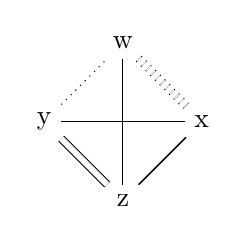
\begin{tikzpicture}
  \node (v0) at (1, 0.) {x};
  \node (v1) at (-1, 0) {y};
  \node (v2) at (0, -1) {z};
  \node (v3) at (0, 1) {w};
  \draw (v0) -- (v1);
  \draw[double, double distance = 0.5ex] (v1) -- (v2);
 \draw[dotted][double, double distance = 0.5ex] (v3) -- (v0);
  \draw (v0) -- (v2);
  \draw (v1) -- (v0);
  \draw[dotted](v1) -- (v3);
  \draw (v2) -- (v0);
  \draw (v2) -- (v3);
  \draw (v3) -- (v2);
\end{tikzpicture}
\caption{Gráfica asociada a  $2wx -2yz - xz - xy - wz + wy$}
\label{figura:1.1}
\end{center}
\end{figure}

\paragraph*{}
Este proceso se puede revertir y asociar a toda gráfica $G$ (posiblemente con aristas punteadas) una forma unitaria que denotaremos por \textbf{$q_{G}$}. Ahora, toda la información de $q_{G}$ está codificada en $G$: La existencia de un vértice $x$ nos dice que la forma cuadrática está definida sobre alguna variable $x$ y que contiene el término $x^{2}$ (porque $q$ es una forma cuadrática unitaria). El coeficiente del monomio $xy$ es $c = a_{p} - a_{s}$ donde $a_{p}$ es la cantidad de aristas punteadas entre $x$ y $y$, y $a_{s}$ es la cantidad de aristas sólidas entre estos mismos vértices. Más aún cabe recalcar que nosotros estamos descartando gráficas con lazos, por lo que cualquier gráfica en verdad define a una forma cuadrática unitaria.\\
Las gráficas de Dynkin se presentan en la figura \ref{figura:1.2}. Denótese que las gráficas $\DynD_{n}$ están definidas para $n \geq 4$ mientras que las gráficas $\DynE_{n}$ solo se definen para $n = 6, 7, 8$. Lo impotante de estas gráficas radica en que permite dar una caracterización elegante de las formas unitarias que son definidas positivas tal como se explica a continuación.

\begin{figure}[H]
\begin{center}
    \begin{tabular}{ll}
    \hline
    Notación \vline & Gráfica\\ 
    \hline
    $\DynA_{n}$, $n\ge1$ &
    \begin{tikzpicture}
    [baseline=(v1.base)]
    \node (v1) at (0, 0) {$1$};
    \node (v2) at (1, 0) {$2$};
    \node (v3) at (4, 0) {$n$};
    \node[draw = none] (v5) at (2.5, 0) {$\ldots$};
    \draw (v1) -- (v2) -- (2, 0);
    \draw (3, 0) -- (v3);
    \end{tikzpicture}\\
    \newline
    $\DynD_{n}$, $n\ge4$ &
    \begin{tikzpicture}
    [baseline=(v1.base)]
    \node (v1) at (0, 0) {$2$};
    \node (v2) at (1, 0) {$3$};
    \node (v3) at (2, 0) {$4$};
    \node (v4) at (5, 0) {$n$};
    \node (v5) at (1, 1) {$1$};
    \node[draw = none] (dots) at (3.5, 0) {$\ldots$};
    \draw (v1) -- (v2) -- (v3) -- (3, 0); \draw (v5)
    -- (v2); \draw (4, 0) -- (v4);
    \end{tikzpicture} \\
    \newline
    $\DynE_{n}$, $n=6$ &
    \begin{tikzpicture} [baseline=(v1.base)]
    \node (v1) at (0, 0) {$2$};
    \node (v2) at (1, 0) {$3$};
    \node (v3) at (2, 0) {$4$};
    \node (v4) at (3, 0) {$5$};
    \node (v5) at (4, 0) {$6$};
    \node (v6) at (2, 1) {$1$};
    \draw (v1) -- (v2) -- (v3) -- (v4);
    \draw (v6) -- (v3);
    \draw (v5) -- (v4);
    \end{tikzpicture}\\
    \newline
    $\DynE_{n}$, $n=7$ &
    \begin{tikzpicture} [baseline=(v1.base)]
    \node (v1) at (0, 0) {$2$};
    \node (v2) at (1, 0) {$3$};
    \node (v3) at (2, 0) {$4$};
    \node (v4) at (3, 0) {$5$};
    \node (v5) at (4, 0) {$6$};
    \node (v7) at (5, 0) {$7$};
    \node (v6) at (2, 1) {$1$};
    \draw (v1) -- (v2) -- (v3) -- (v4);
    \draw (v6) -- (v3);
    \draw (v4) -- (v5);
    \draw (v5) -- (v7);
    \draw (v6) -- (v3);
    \end{tikzpicture}\\
    \newline
    $\DynE_{n}$, $n=8$ &
    \begin{tikzpicture} [baseline=(v1.base)]
    \node (v1) at (0, 0) {$2$};
    \node (v2) at (1, 0) {$3$};
    \node (v3) at (2, 0) {$4$};
    \node (v4) at (3, 0) {$5$};
    \node (v5) at (4, 0) {$6$};
    \node (v7) at (5, 0) {$7$};
    \node (v8) at (6, 0) {$8$};
    \node (v6) at (2, 1) {$1$};
    \draw (v1) -- (v2) -- (v3) -- (v4);
    \draw (v6) -- (v3);
    \draw (v4) -- (v5);
    \draw (v5) -- (v7);
    \draw (v7) -- (v8);
    \end{tikzpicture}
    \end{tabular} 
    \caption{Gráficas de Dynkin. El subíndice $n$ indica la cantidad de vértices que tiene la gráfica.}
    \label{figura:1.2}
\end{center}
\end{figure}

\paragraph*{}
Decimos que la forma unitaria $q$ es \textbf{positiva} si es definida positiva.

\begin{theorem}
Toda forma unitaria $q$ es definida positiva si y solamente si $q$ es $\mathbb{Z}$-equivalente a otra forma unitaria $q'$ donde cada componente conexa de $\textbf{B}_{q'}$ es una gráfica de Dynkin.
\label{teorema:1.6}
\end{theorem}

\paragraph{}
Para poder hacer la demostración hay que comprender el teorema. El teorema dice que la forma unitaria $q(\overrightarrow{x}) = \frac{1}{2}\overrightarrow{x}^{T}A\overrightarrow{x}$ es positiva si y solo si se puede llevar, mediante un cambio de variable entero $\overrightarrow{y} = P\overrightarrow{x}$, a la forma $q'(\overrightarrow{y}) = \frac{1}{2}\overrightarrow{y}^{T}\left(P^{T}~A~P\right)\overrightarrow{y}$ donde $\textbf{B}_{q'}$, tiene la propiedad de que cada una de sus componentes conexas es una gráfica de Dynkin. A dicha gráfica $\textbf{B}_{q'}$ se le llama el \textbf{tipo Dynkin} de $q$.

\begin{example}\citep{AbarcaSoteloMarioAlberto2011Apds}
La forma unitaria
\begin{equation}
    q(w, x, y, z) = x^{2} + y^{2} + z^{2} + w^{2} - xy + yz - yw - zw
    \label{ecuacion:1.5}
\end{equation}\\

tiene asociada la gráfica\\

\begin{center}
\begin{tikzpicture}[scale=1.7]
    \node (v1) at (1.9914399682732804, 0.9921104441137079) {$x$};
    \node (v2) at (0.9905576274421105, 0.7146057713195639) {$y$};
    \node (v3) at (0.0, 0.9512105498862511) {$z$};
    \node (v4) at (0.26505088954607003, 0.0) {$w$};
    \draw (v1) -- (v2);
    \draw[dotted] (v2) -- (v3);
    \draw (v2) -- (v4);
    \draw (v3) -- (v4);
\end{tikzpicture}
\end{center}

y su matriz asociada\\

\begin{center}
\begin{equation*}
    A = \begin{bmatrix}
    2 & -1  &  0 &  0\\
   -1 &  2  &  1 & -1\\
    0 &  1  &  2 & -1 \\
    0 & -1  & -1 &  2
    \end{bmatrix}
\end{equation*}
\end{center}

$P = \begin{bmatrix}
   1 &  0  & 0 & 0\\
   0 &  1  & 0 & 0\\
   0 & -1  & 1 & 0 \\
   0 &  0  & 0 & 1
      \end{bmatrix}$ con inversa  $P^{-1} =  \begin{bmatrix}
   1 &  0  & 0 & 0\\
   0 &  1  & 0 & 0\\
   0 &  1  & 1 & 0 \\
   0 &  0  & 0 & 1
           \end{bmatrix}$
           
\begin{equation*}
\begin{split}
P^{T}~A~P & = \begin{bmatrix}
                1 &  0  &  0 & 0\\
                0 &  1  & -1 & 0\\
                0 &  0  &  1 & 0 \\
                0 &  0  &  0 & 1
             \end{bmatrix}
             \begin{bmatrix}
                2 & -1  &  0 &  0\\
               -1 &  2  &  1 & -1\\
                0 &  1  &  2 & -1 \\
                0 & -1  & -1 &  2
           \end{bmatrix}
           \begin{bmatrix}
                1 &  0  & 0 & 0\\
                0 &  1  & 0 & 0\\
                0 & -1  & 1 & 0 \\
                0 &  0  & 0 & 1
            \end{bmatrix}\\
 & = \begin{bmatrix}
                2 & -1  &  0 &   0\\
               -1 &  1  & -1 &   0\\
                0 &  1  &  2 &  -1 \\
                0 & -1  & -1 &   2
           \end{bmatrix}
           \begin{bmatrix}
                1 &  0  & 0 & 0\\
                0 &  1  & 0 & 0\\
                0 & -1  & 1 & 0 \\
                0 &  0  & 0 & 1
            \end{bmatrix}\\
 & = \begin{bmatrix}
                2 & -1  &   0   &   0\\
               -1 &  2  &  -1  &   0\\
                0 & -1  &   2  &  -1 \\
                0 &  0  &  -1  &   2
           \end{bmatrix}
\end{split}
\end{equation*}

Entonces podemos concluir que $q$ es $\mathbb{Z}$-equivalente a la forma unitaria

\begin{equation*}
q'\left(x, y, z, w\right) = x^{2} + y^{2} + z^{2} + w^{2} - xy - yz - zw
\end{equation*}

con gráfica asociada

\begin{center}
\begin{tikzpicture}[baseline=(v1.base)]
 \centering% El subgrafo está centrado
    \node (v1) at (0, 0) {x};
    \node (v2) at (1, 0) {y};
    \node (v3) at (2, 0) {z};
    \node (v4) at (3, 0) {w};
    \draw (v1) -- (v2);
    \draw (v2) -- (v3); 
    \draw (v3) -- (v4);
\end{tikzpicture}
\end{center}

Esta gráfica es isomorfa a $\mathbb{A}_{4}$, por lo tanto ese es el tipo Dynkin de $q$.
\end{example}

\paragraph{}
Para demostrar el teorema \ref{teorema:1.6} lo dividiremos en dos partes:

\begin{enumerate}
    \item Demostramos que las gráficas de Dynkin son las únicas gráficas conexas de aristas sólidas que definen formas unitarias que son definidas positivas (tomando en cuenta inclusive a las gráficas de aristas múltiples, ver corolario \ref{corolario:1.9}) .
    \item Demostramos que siempre es posible hacer cambios de variable enteros de tal manera que la gráfica resultante no contenga aristas solidas.
\end{enumerate}

El ultimo será demostrado en \ref{sec:2.1}

\begin{lemma}
Las gráficas de Dynkin son las únicas gráficas conexas de aristas sólidas que tienen asociadas formas unitarias positivas.
\label{lema:1.7}
\end{lemma}

\paragraph{}
Para comenzar necesitamos convencernos en verdad de que las gráficas de Dynkin definen formas unitarias positivas. Comencemos con las gráficas de tipo $\DynA_{n}$:

$$x_{1}\rule[1mm]{.1cm}{0.4pt} x_{2} \rule[1mm]{.1cm}{0.4pt}\cdots\rule[1mm]{.1cm}{0.4pt} x_{n}$$

\paragraph{}
Consideremos  la identidad:

\begin{equation*}
    \frac{1}{2}\left(x_{i} - x_{j}\right)^{2} = \frac{1}{2}x_{i}^{2} - x_{i}x_{j} + \frac{1}{2}x_{j}^{2}
\end{equation*}

\paragraph{}
Podemos reescribir la forma unitaria asociada a $\DynA_{n}$ como

\begin{eqnarray*}
 q_{\DynA_{n}}(\overrightarrow{x}) &  =  & \sum_{i=1}^{n}x_{i}^{2} - \sum_{i=1}^{n-1} x_{i}x_{i+1}\\
 &  =  & \frac{1}{2}x_{1}^{2} + \sum_{i=1}^{n-1}\left(\frac{1}{2}x_{i}^{2} + \frac{1}{2} x_{i+1}^{2}\right) + \frac{1}{2}x_{n}^{2} + \sum_{i=1}^{n-1} \left(-x_{i}x_{i+1}\right)\\
 &  =  & \frac{1}{2}x_{1}^{2} + \sum_{i=1}^{n-1}\left(\frac{1}{2}x_{i}^{2} - x_{i}x_{i+1} + \frac{1}{2}x_{i+1}^{2} \right) + \frac{1}{2}x_{n}^{2}\\
 &  =  & \frac{1}{2}x_{i}^{2} + \sum_{i=1}^{n-1}\frac{1}{2}\left(x_{i} - x_{i+1}\right)^{2} + \frac{1}{2}x_{n}^{2}
\end{eqnarray*}

\paragraph{}
Por el teorema \ref{teorema:1.4} se concluye que $q_{\DynA_{n}}$ es definida positiva. La demostración para la forma unitaria $q_{\DynD_{n}}$ es similar solo que en este caso se usa la identidad:

\begin{equation*}
    \frac{1}{2}\left[\left(x_{3} - x_{2} - x_{1}\right)^{2} + \left(x_{2} - x_{1}\right)^{2}\right] = x_{1}^{2} + x_{2}^{2} + \frac{1}{2}x_{3}^{2} - x_{1}x_{3} - x_{2}x_{3}
\end{equation*}

\paragraph{}
de tal forma que 

\begin{eqnarray*}
 q_{\DynD_{n}}(\overrightarrow{x}) &  =  & \sum_{i=1}^{n}x_{i}^{2} - x_{1}x_{3} -  \sum_{i=2}^{n-1} x_{i}x_{i+1}\\
 &  =  & \frac{1}{2}\left[\left(x_{3} - x_{2} - x_{1}\right)^{2} + \left(x_{2} - x_{1}\right)^{2} + \sum_{i=3}^{n-1}\left(x_{i} - x_{i+1}\right)^{2}  + x_{n}^{2}\right]
\end{eqnarray*}. 

\paragraph{}
Para las gráficas $\DynE_{6}$, $\DynE_{7}$ y $\DynE_{8}$ usaremos el siguente razonamiento:\\
Supongamos que $A_{\Delta}$ es la matriz asociada a la gráfica $\Delta$ (con $\Delta = \DynE_{6},\DynE_{7},\DynE_{8}$); si existe una matriz $R_{\Delta}$ tal que $A_{\Delta} = R_{\Delta}^{T}R_{\Delta}$ entonces por teorema \ref{teorema:1.5} se sigue que $\Delta$ define una forma unitaria definida positiva.\\
En efecto tenemos que:

\begin{align*}
 A\DynE_{6} &  =  \begin{bmatrix}
 2 & 0 & 0 & -1 & 0 & 0\\
 0 & 2 & -1 & 0 & 0 & 0\\
 0 & -1 & 2& -1 & 0 & 0\\
 -1 & 0 & -1 & 2 & -1 & 0\\
 0 & 0 & 0 & -1 & 2 & -1\\
 0 & 0 & 0 & 0 & -1 & 2\\
 \end{bmatrix}\\
 R\DynE_{6} &  =   \begin{bmatrix}
 \sqrt{2} & 0 & 0 & -\frac{1}{\sqrt{2}} & 0 & 0\\
 0 & sqrt(2) & - \frac{1}{\sqrt{2}}& 0 & 0 & 0\\
 0 & 0 & \frac{\sqrt{3}}{\sqrt{2}} & -\frac{\sqrt{2}}{\sqrt{3}} & 0 & 0\\
 0 & 0 & 0 & \frac{\sqrt{5}}{\sqrt{6}} & -\frac{\sqrt{6}}{\sqrt{5}} & 0\\
 0 & 0 & 0 & 0 & \frac{2}{\sqrt{5}} & -\frac{\sqrt{5}}{2}\\
 0 & 0 & 0 & 0 & 0 & \frac{\sqrt{3}}{2}\\
 \end{bmatrix}
 \end{align*}\\

 \begin{align*}
 A\DynE_{7} &  =  \begin{bmatrix}
 2 & 0 & 0 & -1 & 0 & 0 & 0\\
 0 & 2 & -1 & 0 & 0 & 0 & 0\\
 0 & -1 & 2 & -1 & 0 & 0 & 0\\
 -1 & 0 & -1 & 2 & -1 & 0 & 0\\
 0 & 0 & 0 & -1 & 2 & -1 & 0\\
 0 & 0 0 & 0 & 0 & -1 & 2 & -1\\
 0 & 0 & 0 & 0 & 0 & -1 & 2\\
 \end{bmatrix}\\
 R\DynE_{7} &  =  \begin{bmatrix}
 \sqrt{2} & 0 & 0 & -\frac{1}{\sqrt{2}} & 0 & 0 & 0 & 0\\
 0 & sqrt(2) & - \frac{1}{\sqrt{2}}& 0 & 0 & 0 & 0 & 0\\
 0 & 0 & \frac{\sqrt{3}}{\sqrt{2}} & -\frac{\sqrt{2}}{\sqrt{3}} & 0 & 0 & 0 & 0\\
 0 & 0 & 0 & \frac{\sqrt{5}}{\sqrt{6}} & -\frac{\sqrt{6}}{\sqrt{5}} & 0 & 0 & 0\\
 0 & 0 & 0 & 0 & \frac{2}{\sqrt{5}} & -\frac{\sqrt{5}}{2} & 0 & 0\\
 0 & 0 & 0 & 0 & 0 & \frac{\sqrt{3}}{2} & -\frac{2}{\sqrt{3}}\\
 0 & 0 & 0 & 0 & 0 & 0 & 0 & \frac{\sqrt{2}}{\sqrt{3}}\\
 \end{bmatrix}
 \end{align*}\\

 \begin{align*}
 A\DynE_{8} &  = \begin{bmatrix}
 2 & 0 & 0 & -1 & 0 & 0 & 0 & 0\\
 0 & 2 & -1 & 0 & 0 & 0 & 0 & 0\\
 0 & -1 & 2 & -1 & 0 & 0 & 0 & 0\\
 -1 & 0 & -1 & 2 & -1 & 0 & 0 & 0\\
 0 & 0 & 0 & -1 & 2 & -1 & 0 & 0 \\
 0 & 0 & 0 & 0 & -1 & 2 & -1 & 0\\
 0 & 0 & 0 & 0 & 0 & -1 & 2 & -1\\
 0 & 0 & 0 & 0 & 0 & 0 & -1 & 2\\
 \end{bmatrix}
\end{align*}

\begin{align*}
 R\DynE_{8} &  = \begin{bmatrix}
 \sqrt{2} & 0 & 0 & -\frac{1}{\sqrt{2}} & 0 & 0 & 0 & 0 & 0\\
 0 & sqrt(2) & - \frac{1}{\sqrt{2}}& 0 & 0 & 0 & 0 & 0 & 0\\
 0 & 0 & \frac{\sqrt{3}}{\sqrt{2}} & -\frac{\sqrt{2}}{\sqrt{3}} & 0 & 0 & 0 & 0 & 0\\
 0 & 0 & 0 & \frac{\sqrt{5}}{\sqrt{6}} & -\frac{\sqrt{6}}{\sqrt{5}} & 0 & 0 & 0 & 0\\
 0 & 0 & 0 & 0 & \frac{2}{\sqrt{5}} & -\frac{\sqrt{5}}{2} & 0 & 0 & 0\\
 0 & 0 & 0 & 0 & 0 & \frac{\sqrt{3}}{2} & -\frac{2}{\sqrt{3}} & 0 & 0\\
 0 & 0 & 0 & 0 & 0 & 0 & 0 & \frac{\sqrt{2}}{\sqrt{3}} & - \frac{\sqrt{3}}{\sqrt{2}}\\
 0 & 0 & 0 & 0 & 0 & 0 & 0 & \frac{1}{\sqrt{2}} & 0\\
 \end{bmatrix}
\end{align*}

\paragraph{}
Aun no hemos terminado la demostración del lema \ref{lema:1.7} . Falta demostrar que las gráficas de Dynkin son las únicas gráficas de aristas sólidas que definen formas unitarias positivas. Comenzaremos con el siguiente lema, el cual muestra que toda gráfica que tenga aristas múltiples no corresponde a ninguna forma unitaria positiva.

\begin{lemma}
Si la forma unitaria $q(\overrightarrow{x})$ es positiva entonces $q_{ij} \in \{-1,0,1\}$ para todo $1\leq i \le j \leq n$.
\label{lema:1.8}
\end{lemma}

\begin{proof}
Denotemos con $ \overrightarrow{e}_{k} = \left(d_{1},d_{2}, \ldots , d_{n}\right)$ al vector dado por $d_{k} = 1$ y $d_{i} = 0$ para toda $i\neq k$. Si $q_{ij} \geq 2$ entonces $q(\overrightarrow{e}_{i} + \overrightarrow{e}_{j}) = 2 - q_{ij} \leq 0$ pero $\overrightarrow{e}_{i} - \overrightarrow{e}_{j} \neq \overrightarrow{0}$. Si $q_{ij} \leq -2$ entonces $q\left(\overrightarrow{e}_{i}+ \overrightarrow{e}_{j}\right) = 2 - q_{i,j} \leq 0$ pero $\overrightarrow{e}_{i} - e_{j} \neq \overrightarrow{0}$. De lo anterior, ya que $q$ es definida positiva, entonces $|q_{ij}| \le 2$ para todo $1 \leq i \le j \leq n$.
\end{proof}

\paragraph{}
Cada $|q_{ij}|$ nos dice la cantidad de aristas que hay entre los vértices $x_{i}$ y $x_{j}$ de la gráfica $\textbf{B}_{q}$; por lo tanto si $|q_{ij}| \leq 1$ tenemos que $\textbf{B}_{q}$ es una gráfica simple. Es decir que el lema \ref{lema:1.8} se puede reescribir como sigue:

\begin{corollary}
Si $q$ es una forma unitaria positiva entonces necesariamente $\textbf{B}_{q}$ es una gráfica simple.
\label{corolario:1.9}
\end{corollary}

\paragraph{}
Con base en este corolario diremos que una forma unitaria $q$ es \textbf{simple} si su gráfica asociada $\textbf{B}_{q}$ es una gráfica simple.\\
Ahora que hemos descartado a las gráficas de aristas multiples (a las pseudográficas que tienen lazos sencillamente no se consideran en este trabajo) el resto de la demostración es como sigue:

\begin{enumerate}
    \item Demostraremos que toda gráfica que contenga a una gráfica Euclidiana (Figura \ref{figura:1.3}) no define a una forma unitaria positiva
    \item Demostraremos que toda gráfica conexa que no sea de Dynkin necesariamente contiene una subgráfica Euclidiana
\end{enumerate}

\begin{figure}
    \centering
    \begin{tabular}{ll}
    \hline
    Notación \vline & Gráfica\\ 
    \hline
    $\widetilde{\DynA_{m}}$&
    \begin{tikzpicture}[baseline=(v1.base)]
  \node (v0) at (0.16, -0.76) {};
  \node (v1) at (-1.0, -0.79) {};
  \node (v2) at (-1.56, 0.23) {};
  \node (v3) at (-0.97, 1.24) {};
  \node (v4) at (0.19, 1.26) {};
  \node (v5) at (0.74, 0.24) {};
  \draw (v0) -- (v1);
  \draw (v1) -- (v2);
  \draw (v2) -- (v3);
  \draw (v3) -- (v4);
  \draw (v4) -- (v5);
  \draw[dotted] (v5) -- (v0);
    \end{tikzpicture}\\
    \newline
    $\widetilde{\DynD_{m}}$ &
    \begin{tikzpicture}[baseline=(v1.base)]
    \node (v1) at (0, 0) {};
    \node (v2) at (1, 0) {};
    \node (v3) at (2, 0) {};
    \node (v4) at (5, 0) {};
    \node (v5) at (1, 1) {};
    \node (v6) at (6, 0) {};
    \node (v7) at (5, 1) {};
    \node[draw = none] (dots) at (3.5, 0) {$\ldots$};
    \draw (v1) -- (v2) -- (v3) -- (3, 0); 
    \draw (v5) -- (v2); 
    \draw (4, 0) -- (v4); 
    \draw (v4) -- (v6); 
    \draw (v4) -- (v7);
    \end{tikzpicture}\\
    \newline
    $\widetilde{\DynE_{6}}$ &
    \begin{tikzpicture} [baseline=(v1.base)]
    \node (v1) at (0, 0) {};
    \node (v2) at (1, 0) {};
    \node (v3) at (2, 0) {};
    \node (v4) at (3, 0) {};
    \node (v5) at (4, 0) {};
    \node (v6) at (2, 1) {};
    \node (v7) at (2, 2) {};
    \draw (v1) -- (v2) -- (v3) -- (v4);
    \draw (v6) -- (v3);
    \draw (v5) -- (v4);
    \draw (v6) -- (v7);
    \end{tikzpicture}\\
    \newline
    $\widetilde{\DynE_{7}}$ &
    \begin{tikzpicture} [baseline=(v1.base)]
    \node (v1) at (0, 0) {};
    \node (v2) at (1, 0) {};
    \node (v3) at (2, 0) {};
    \node (v4) at (3, 0) {};
    \node (v5) at (4, 0) {};
    \node (v7) at (5, 0) {};
    \node (v6) at (2, 1) {};
    \node (v8) at (-1, 0) {};
    \draw (v1) -- (v2) -- (v3) -- (v4);
    \draw (v6) -- (v3);
    \draw (v4) -- (v5);
    \draw (v5) -- (v7);
    \draw (v8) -- (v3);
    \end{tikzpicture}\\
    \newline
    $\widetilde{\DynE_{8}}$&
    \begin{tikzpicture} [baseline=(v1.base)]
    \node (v1) at (0, 0) {};
    \node (v2) at (1, 0) {};
    \node (v3) at (2, 0) {};
    \node (v4) at (3, 0) {};
    \node (v5) at (4, 0) {};
    \node (v7) at (5, 0) {};
    \node (v8) at (6, 0) {};
    \node (v6) at (2, 1) {};
    \node (v9) at (7, 0) {};
    \draw (v1) -- (v2) -- (v3) -- (v4);
    \draw (v6) -- (v3);
    \draw (v4) -- (v5);
    \draw (v5) -- (v7);
    \draw (v7) -- (v8);
    \draw (v9) -- (v8);
    \end{tikzpicture}
    \end{tabular} 
    \caption{Gráficas Euclidianas. La cantidad de vértices que tiene cada gráfica es $n = m + 1$.}
    \label{figura:1.3}
\end{figure}

\paragraph{}
Hasta ahora hemos asociado vértices con variables(\begin{tikzpicture}\node (v1) at (-0.0, 0.56) {x}; \end{tikzpicture} con x) pero vamos a extender el concepto de la siguiente manera: si en lugar de etiquetar con variables etiquetamos con números enteros(\begin{tikzpicture}\node (v1) at (-0.0, 0.56) {2}; \end{tikzpicture} con 2), convenimos que estamos evaluando la variable correspondiente a dicho número.

\begin{example}
Consideremos la forma cuadrática asociada a \ref{ecuacion:1.5}; entonces la gráfica representa la evaluación $x = 2$, $y=1$, $z=2$, $w=-1$, es decir

\begin{align*}
q(2, 1, 2, -1) &  = 2^{2} + 1^{2} + 2^{2} + (-1)^{2} + 2\cdot 1 + 2\cdot(-1) - 2\cdot1 - 1\cdot(-1) - 2\cdot(-1) - 2\cdot 2 \\
               &  = 7
\end{align*}
\end{example}

\paragraph{}
Usando esta notación mostraremos que si $\textbf{B}_{q}$ contiene una subgráfica Euclidiana entonces existe un vector $\overrightarrow{x} \neq 0$ tal que $q\left(\overrightarrow{x}\right) = 0$, mostrando así que $q(\overrightarrow{x})$ no es definida positiva. Este vector se construye de la siguiente manera: se evalúan todas las variables que corresponden a la subgráfica Euclidiana de acuerdo a la figura \ref{figura:1.4} y todas las demas variables se evalúan a cero. Un simple cálculo nos muestra que esta evaluación produce un vector $\overrightarrow{x} \neq \overrightarrow{0}$ tal que $q\left(\overrightarrow{x}\right) = 0$.\\


\begin{figure}[h]
    \begin{subfigure}[b]{0.5\textwidth}
        \begin{minipage}{7cm}
        \centering% El subgrafo está centrado
        \begin{tikzpicture}
        \node (v0) at (1.56, 0.14) {1};
        \node (v1) at (1.02, 1.11) {1};
        \node (v2) at (-0.07, 1.31) {1};
        \node (v3) at (-0.91, 0.58) {1};
        \node (v4) at (-0.89, -0.54) {1};
        \node (v5) at (0.01, -1.16) {1};
        \node (v6) at (1.07, -0.86) {1};
        \draw (v0) -- (v1);
        \draw (v1) -- (v2);
        \draw (v3) -- (v2);
        \draw (v3) -- (v4);
        \draw (v4) -- (v5);
        \draw (v5) -- (v6);
        \draw[dotted] (v6) -- (v0);
        \end{tikzpicture}
        \end{minipage}
        \caption{Raíz de $\widetilde{\DynA}_{m}$}
     \end{subfigure}
     \begin{subfigure}[b]{0.5\textwidth}
        \begin{minipage}{7cm}
        \centering% El subgrafo está centrado
        \begin{tikzpicture}
        \node (v0) at (0.17, -0.93) {1};
        \node (v1) at (1.27, -0.93) {2};
        \node (v2) at (2.37, -0.93) {3};
        \node (v3) at (3.47, -0.93) {4};
        \node (v4) at (3.47, 0.73) {5};
        \node (v5) at (4.57, -0.93) {6};
        \node (v6) at (5.67, -0.93) {7};
        \node (v7) at (6.77, -0.93) {8};
        \draw (v0) -- (v1);
        \draw (v1) -- (v2);
        \draw (v2) -- (v3);
        \draw (v3) -- (v4);
        \draw (v3) -- (v5);
        \draw (v6) -- (v7);
        \draw (v5) -- (v6);
        \end{tikzpicture}
        \end{minipage}
        \caption{Raíz de $\widetilde{\DynE}_{7}$}
     \end{subfigure}
     \begin{subfigure}[b]{0.5\textwidth}
        \begin{minipage}{7cm}
        \centering% El subgrafo está centrado
        \begin{tikzpicture}
        \node (v0) at (3.47,  1.93) {1};
        \node (v1) at (1.27, -0.93) {2};
        \node (v2) at (2.37, -0.93) {3};
        \node (v3) at (3.47, -0.93) {4};
        \node (v4) at (3.47, 0.43) {5};
        \node (v5) at (4.57, -0.93) {6};
        \node (v6) at (5.67, -0.93) {7};
        \draw (v0) -- (v4);
        \draw (v1) -- (v2);
        \draw (v2) -- (v3);
        \draw (v3) -- (v4);
        \draw (v3) -- (v5);
        \draw (v5) -- (v6);
        \end{tikzpicture}
        \end{minipage}
        \caption{Raíz de $\widetilde{\DynE}_{6}$}
     \end{subfigure}
     \begin{subfigure}[b]{0.5\textwidth}
        \begin{minipage}{7cm}
        \centering% El subgrafo está centrado
        \begin{tikzpicture}
        \node (v0) at (7.87, -0.93) {1};
        \node (v1) at (1.27, -0.93) {2};
        \node (v2) at (2.37, -0.93) {3};
        \node (v3) at (3.47, -0.93) {4};
        \node (v4) at (3.47, 0.73) {5};
        \node (v5) at (4.57, -0.93) {6};
        \node (v6) at (5.67, -0.93) {7};
        \node (v7) at (6.77, -0.93) {8};
        \node (v8) at (8.97, -0.93) {9};
        \draw (v0) -- (v7);
        \draw (v1) -- (v2);
        \draw (v2) -- (v3);
        \draw (v3) -- (v4);
        \draw (v3) -- (v5);
        \draw (v6) -- (v7);
        \draw (v5) -- (v6);
        \draw (v0) -- (v8);
        \end{tikzpicture}
        \end{minipage}
        \caption{Raíz de $\widetilde{\DynD}_{m}$}
     \end{subfigure}
     \begin{center}
      \begin{subfigure}[b]{0.8\textwidth}
        \centering% El subgrafo está centrado
        \begin{tikzpicture}
        \node (v0) at (1.27, 0.83) {1};
        \node (v1) at (1.27, -0.73) {2};
        \node (v2) at (2.37, -0.13) {3};
        \node (v3) at (3.47, -0.13) {4};
        \node (v4) at (6.27, -0.13) {5};
        \node (v5) at (7.37, -0.73) {6};
        \node (v6) at (7.37, 0.83) {7};
        \node[draw = none] (dots) at (4.87, -0.13) {$\ldots$};
        \draw (v0) -- (v2);
        \draw (v1) -- (v2);
        \draw (v2) -- (v3) -- (4.57, -0.13);
        \draw (5.17, -0.13) -- (v4) -- (v5);
        \draw (v4) -- (v6);
        \end{tikzpicture}
        \caption{Raíz de $\widetilde{\DynE}_{8}$}
      \end{subfigure}
     \end{center}
     \caption{Raíces de las formas unitarias asociadas a las gráficas Euclidianas.}
    \label{figura:1.4}
\end{figure}

Solamente falta demostrar que toda gráfica que no sea de Dynkin necesariamente contiene a una subgráfica Euclidiana. Sea $G$ una gráfica conexa de $n$ vértices distinta de $\DynA_{n} \DynD_{n}, \DynE_{6}, \DynE_{7} ~y~ \DynE_{8}$. Si $G$ no es un árbol entonces $G$ contiene un ciclo; es decir contiene una subgráfica de $\widetilde{\DynA}_{m}$ para algún $m < n$. Si $G$ es un árbol, y dado que $G\neq \DynA_{n}$, entonces existe al menos un vértice $v$ de grado 3 o más. Claramente $v$ pertenece a una subgráfica de $\DynD_{r}$ para algún $r \leq n$, pero habíamos supuesto que $G \neq \DynD_{n}$ por lo tanto hay tres casos:

\begin{enumerate}
    \item Si $v$ tiene grado estrictamente mayor a 3 entonces $G$ contiene a $\widetilde{D}_{4}$
    \item Si $G$ contiene otro vértice $w$ de grado 3 o más, entonces $G$ contiene a $\widetilde{D}_{m}$ para algún $m < n$
    \item Si todos los demás vértices tienen grado menor a 3 entonces $G$ debe contener a $\DynE_{6}$ como subgráfica.
\end{enumerate}

\paragraph{}
 Ahora ya que habiamos supuesto que $G \neq \DynE_{6}$, por tanto $n > 6$. Eneste caso $G$ debe contener a $\widetilde{\DynE}_{6}$ o $\DynE_{7}$. Si tenemos que $G = \DynE_{7}$ entonces $n > 8$., de donde obtenemos que $G$ contiene a $\widetilde{\DynE}_{7}$ o $\DynE_{8}$, pero si $G \neq \DynE_{8}$ entonces $n > 8$ y por lo tanto $G$ contiene a $\widetilde{\DynE}_{8}$.\\
Resumiendo, las gráficas de Dynkin definen formas unitarias positivas, y cualquier otra gráfica conexa y de aristas solidas que no sea de Dynkin necesariamente contiene una gráfica Euclidiana que la vuelve no positiva: por lo tanto las gráficas de Dynkin son las únicas gráficas conexas de aristas sólidas que definen formas unitarias positivas. Esto conluye la demostración del lema \ref{lema:1.7}.\\
En la sección \ref{sec:2.1} se dará termino a la demostración del teorema \ref{teorema:1.6}
